\chapter{Design} \label{cap:cap3}

\section{Persistance design}
Our system needs to store and retrieve persistent data, to achieve this task we decide to use PostgreSQL free RDBMS. In the following paragraph~\ref{sec:er} we will analyze the design of our database.
\subsection{ER Diagram}\label{sec:er}
In order to understand the organization and the design of our database we will describe and analyze it through the use of the Entity-Relationship Diagram in figure~\ref{fig:er}.
The main entity of the database are four:
\begin{itemize}
\item{\bf User}: it represents the data of a registered user and contains all his information such as the email, the first name, the surname, the username and the password. It's in a relationship "one to many" with the \textit{Calendar} entity because we assume that in a future our users may have one or more calendar and not only a single agenda.
\item{\bf Calendar}: it stands for the agenda of the user, its only attribute is a boolean that indicates whether is public or not. It's related with the \textit{User} and the \textit{Event} entity. It's in a "one to one" relationship with the User because a calendar belongs only to an unique User. Conversely the relationship with the \textit{Event} entity could be of two different type, \textit{Participation} or \textit{Owner}. The first one is a relationship "zero to many" because it could have either no participant or many participant to it. The second, instead, is a "one to many" relationship because an event needs at least one owner that had previously created it and eventually it can have more owner that can manage it, even if this aspect will not be part of our first release but it's scheduled for a later release.
\item{\bf Event}: it represents the information intrinsic stored such as its participants, the place, the date etc.. Since it is associated to his owner \textit{Calendar} and, possibly, to his participants' \textit{Calendars}, its participant can be zero but the owner must be at least one. Therefore the event must be related through an "one to many" relationship with the \textit{Calendar}. Additionally it is in relation "zero to many" with the \textit{WeatherStateConstraint} because it can have different constraints, like "it must be sunny or cloudy".
\item{\bf WeatherContraint}: it stands for the constraint associated to an Event such as the temperature. It's in a relation "one to one" with an Event, because any WeatherConstraint belong exactly to one Event but is in a relation "1 to many" with the WeatherStateConstraint that represent the desired weather condition of an event such as sunny, cloudy , rainy and so on, in fact any user has the possibility to choose different desired condition when creating a new event.
\end{itemize}
 \begin{center}
 \begin{figure}[H]
    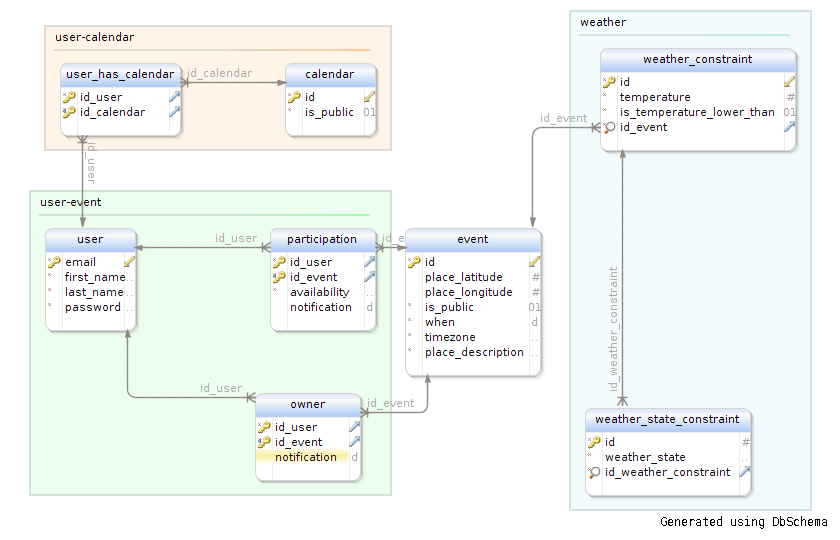
\includegraphics[width=1\textwidth]{../ERDiagram/er/er.png}
    \caption{ER Diagram}
     \label{fig:er}
     \end{figure}
   \end{center}  
\section{Modeling}
In this section is illustrated the modeling process through that we try to understand how to implement in the best possible way a good and well designed architecture in order to develop a robust  and  safe system. We use various pattern to achieve this goals: \begin{itemize}
\item BCE Pattern
\item MVC Pattern
\item Sequence Diagram
\end{itemize}
\subsection{Structure}
\subsubsection{Server-side BCE}\label{sec:BCE}
This paragraph illustrates the BCE pattern representing the architecture that we'll implement in order to develop the WeatherCal system. When identifying the elements for some scenarios of system behavior, we can align each participating element with one of three key perspectives: Boundary, Control and Entity. \\This  pattern is a variation of the MVC pattern indeed we can consider mapping the Boundary with the MVC's View, the Control with the MVC's Controller and the Entity with the MVC's Model. Moreover the BCE pattern is not solely appropriate for dealing with user interfaces but it gives also to the controller a slightly different role to play.\\Let's take a deeper look in to the BCE pattern:\begin{itemize}
\item Entity: are objects representing system data and also they perform behavior organized around some cohesive amount of data.
\item Boundaries: are the objects that interface with system actors and most of the times they lay on periphery of a system. Some boundary elements will be "front-end" elements that accept input from outside the area under design and other elements will be "back-end" managing communication to supporting elements outside the system or subsystem.
\item Control: are the elements that mediate between boundaries and entities and control the flow of the interaction of the scenario. They manage the execution of commands coming from the boundary.
\myparagraph{Entity overview}
The diagram in~\ref{fig:entityovervie} illustrates an overview of all entities involved in our system and how they are related with each other.
 \begin{center}
 \begin{figure}[H]
    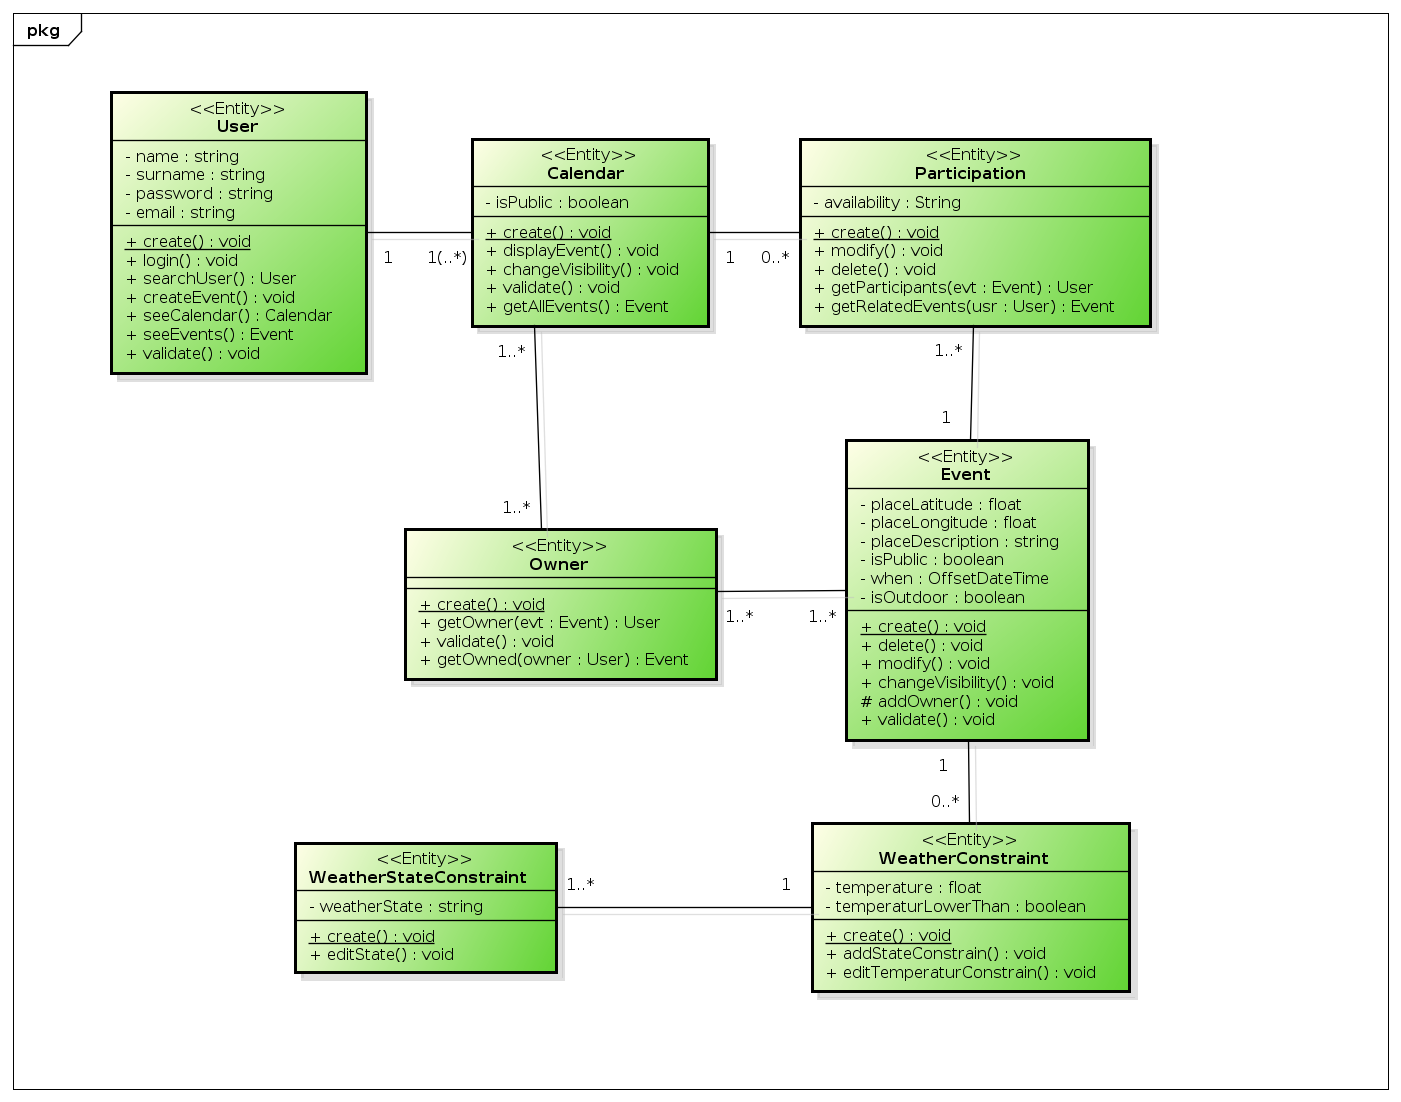
\includegraphics[width=1\textwidth]{../BCEDiagram/BCE/EntityOverview/Entity.png}
    \caption{Entities involved}
     \label{fig:entityovervie}
     \end{figure}
   \end{center}  


\myparagraph{Sign Up and Log In}
The diagram in~\ref{fig:logBCE} shows the flow of the system's behavior related to the registered user's login or to the anonymous user's signup. After the SignUp Controller validates the values submitted by the user, the user reaches his UserPage and then the CalendarController loads its agenda and all associated event. \\In these diagram there are three entities who plays an active role:
\begin{enumerate}
\item  {\bf User}: it's a registered user that can log in to the platform and gets to his UserPage, or he can represents someone who is not already signed in  to the system and can only reach the main page and register to the platform.
\item  {\bf Event}: represents an event in the calendar. An user can be related to it in two different way, it could be a guest or it could be its owner. Depending on this relation it can perform different action. He can modifies it or creates a new one if he's his owner or change his participation if he's a guest.
\item  {\bf Calendar}: is an element that represents the agenda of an user and contains all his scheduled event. It can be set public or private by its owner.
\end{enumerate}
There are two boundaries involved in this scenario: \begin{enumerate}
\item {\bf MainPage}: it represents the index page of the system. The one in which a user can either log in or sign up to the platform.
\item {\bf UserPage}: it stands for the page reached by the user after he logged in. It shows his calendar and all other tasks that the user can performs within it, such as searches for a user, creates or modifies an event or checks for notification.
 \end{enumerate}
The controls who manage the flow of this scenario are two:\begin{enumerate}
\item {\bf SignUpController}: it's the control whose role is to handle the registration's request of a new user into the system. Whenever a non registered user submits his information the SignUpController verifies the correctness of these information and if they are valid it creates a new User and redirect him to the UserPage.
\item {\bf LoginController}: his task is to manage the log in of a registered user. It verifies that the credentials submitted by the user are the same provided in the system registration.  
\item {\bf CalendarController}: It's the responsible for the control of the calendar of an user, it loads it and all its associated events, through it an user can search other users' calendar and view them if they were set as public by their owner.
\end{enumerate}
\begin{center}
 \begin{figure}[H]
    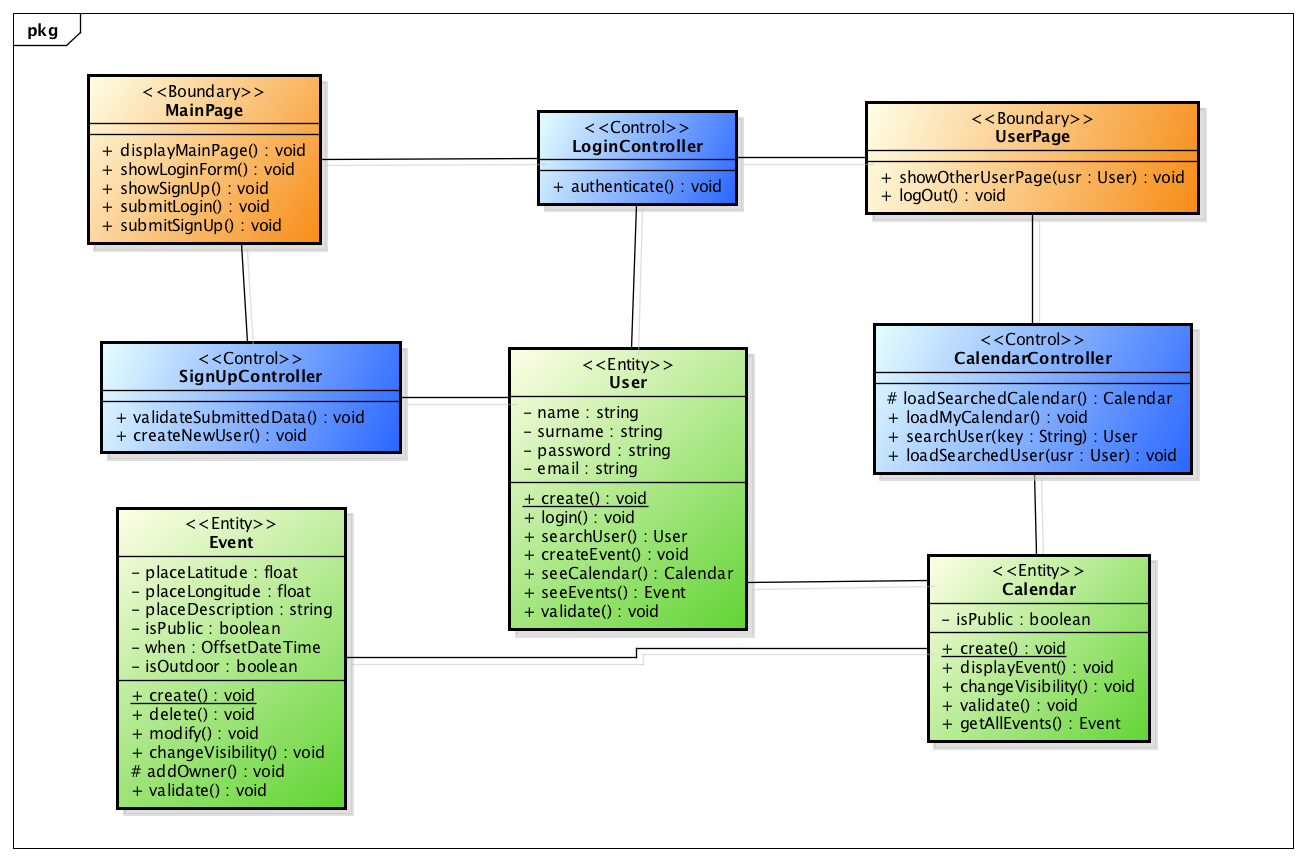
\includegraphics[width=1\textwidth]{../BCEDiagram/BCE/EntityOverview/LoginBCE.png}
    \caption{Sign Up and Log In}
     \label{fig:logBCE}
     \end{figure}
   \end{center}  
\end{itemize}

\myparagraph{Event creation or modification}
The diagram in~\ref{fig:editneweventBCE} illustrates the flow of the creation of the modification of an event. Naturally an user can perform these action only if it's logged in to the system. The top side of the diagram it's related to the log in mechanism already seen in fig~\ref{fig:logBCE} while the bottom side represents the management of an event. From that point on through the EventController a user can either create,delete or modify an event, see the event information or change the participation to it.
\\In these diagram there are only two entities who plays an active role:
\begin{enumerate}
\item {\bf User}: it's a registered user that can log in to the platform and gets to his UserPage, or he can represents someone who is not already signed in to the system and can only reach the main page and register to the platform.
\item {\bf Event}: represents an event in the calendar. An user can be related to it in two different way, it could be a guest or it could be its owner. Depending on this relation it can perform different action. Modify or create it if it's an owner or change his participation if it's a guest.
\end{enumerate}
There are two boundaries involved in this scenario: \begin{enumerate}
\item {\bf UserPage}: it stands for the page reach by the user after he logged in. It shows his calendar and all other tasks that the user can performs within it such as searches for a user, creates or modifies an event or checks for notification.
\item {\bf NewModifyEventPage}: is the page that a user uses to create or manipulate an event. It displays all the informations about the selected event such as the place, the date and the desired weather. More over gives to the owner of the event the capability to modify these data or to insert new informations in case that the user is creating a new event.
 \end{enumerate}
The controls who manage the flow of this scenario are two:\begin{enumerate}
\item {\bf LoginController}: his task is to manage the log in of a registered user. It verifies that the credentials submitted by the user are the same provided in the system registration.  
\item {\bf EventController}: this control has several duties many of which concerning the event creation or modification. It's able either to load the information regarding an existing event, to delete an event or to check the correctness of the submitted values for its attributes when the event is created. In addition an invited user to the event can eventually changes the participation to it.
\end{enumerate}
\begin{center}
 \begin{figure}[H]
    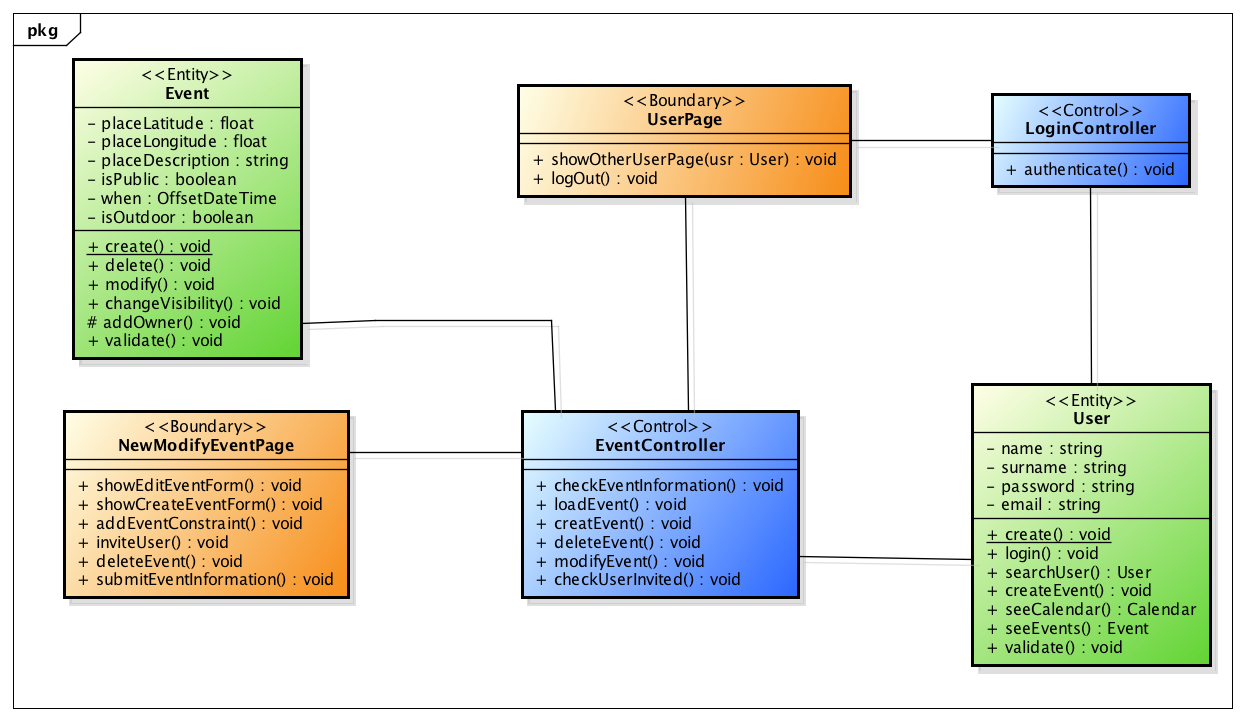
\includegraphics[width=1\textwidth]{../BCEDiagram/BCE/EntityOverview/EventManagementBCE.png}
    \caption{Create or modify an event}
     \label{fig:editneweventBCE}
     \end{figure}
   \end{center}  
\myparagraph{Search Users}
The diagram in fig~\ref{fig:searchBCE} display the scenario involved when a user searches for an other user profile. The flow depends also by the visibility of both the searched calendar and the events within it. This action of course can only be performed by a logged user.\\
In these diagram there are three entities:
\begin{enumerate}
\item {\bf User}: it's a registered user that can log in to the platform and gets to his UserPage, or he can represents someone who is not already signed in to the system and can only reach the main page and register to the platform.
\item {\bf Event}: represents an event in the calendar. A user can be related to it in two different way, it could be a guest or it could be its owner. Depending on this relation it can perform different action. Modify or create it if it's an owner or change his participation if it's a guest.
\item {\bf Calendar}: is an element that represents the agenda of an user and contains all his scheduled event. It can be set public or private by its owner.
\end{enumerate}
There are two boundaries involved in this scenario: \begin{enumerate}
\item {\bf UserPage}: it stands for the page reached by the user after he logs in. It shows his calendar and all other tasks that the user can performs within it such as searches for a user, creates or modifies an event or checks for notification.
 \item {\bf OtherUserCalendarPage}: is the page that an user can reach after he searched for an other user, depending on the searched user's calendar's visibility it can shows either the calendar itself and its related event or a redirect to the home page
 \end{enumerate}
The controls who manage the flow of this scenario it's unique:\begin{enumerate}
\item {\bf CalendarController}: It's the responsible for the control of the calendar of an user, it loads it and all its associated events, through it an user can search other users' calendar and view them if they were set as public by their owner.

\end{enumerate}
\begin{center}
 \begin{figure}[H]
    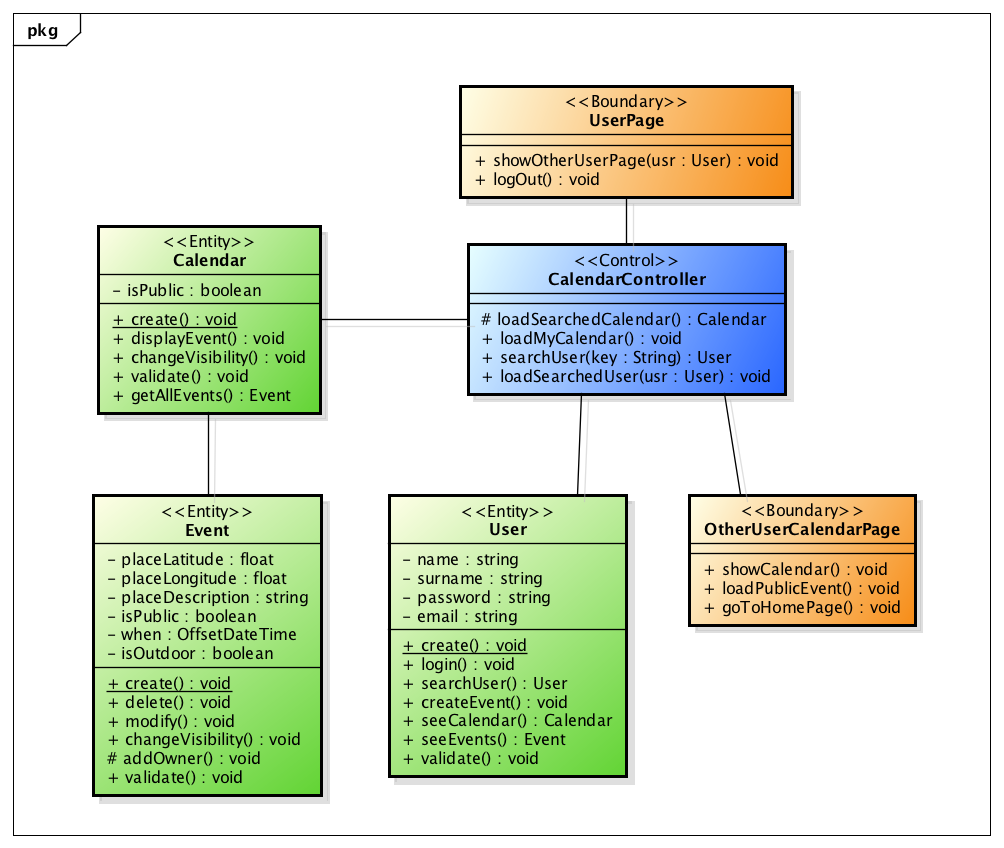
\includegraphics[width=1\textwidth]{../BCEDiagram/BCE/EntityOverview/SearchUserBCE.png}
    \caption{Search users}
     \label{fig:searchBCE}
     \end{figure}
   \end{center} 
  
  
\subsubsection{Client-side MVC}
An other part of the architecture, located on the client side will rely on an MVC framework as stated in \autoref{sec:sec2.3}.
In this paragraph the diagrams implementing the structure of the client side application are described.\\
We will have three categories of system element: \textit{Model} elements, \textit{View} elements and \textit{Controller} elements.
\begin{itemize}
\item \textbf{Model elemens} will be composed by two classes,\textit{Collections} and \textit{Models}, the former implementing a set of the latters.
\item \textbf{View elements} have similar differencies, even if weaker. \textit{ItemViews} will mostly be used for displaying collections, even if they were thought for displaying single elements. Anyway, since any operation should be performed on the collection and the models contain few data, they can be used even for displaying collections. Even though, collections are usually rendered with \textit{CollectionViews}, a sort of "set of \textit{ItemViews}".
\item \textbf{Controller elements} does not exactly exist both in the diagrams and in the framework. This is because there is no need of a real controller. Its job will be accomplished by the Application entry point, in such a way that can be associated to the Controller of the MVC pattern, but just in a coarse approximation.
\end{itemize}
\myparagraph{Entity overview}
The diagram in~\ref{fig:modelovervie} illustrates an overview of all the models and the collections which are part of the system and how they interact among themselves.
 \begin{center}
 \begin{figure}[H]
    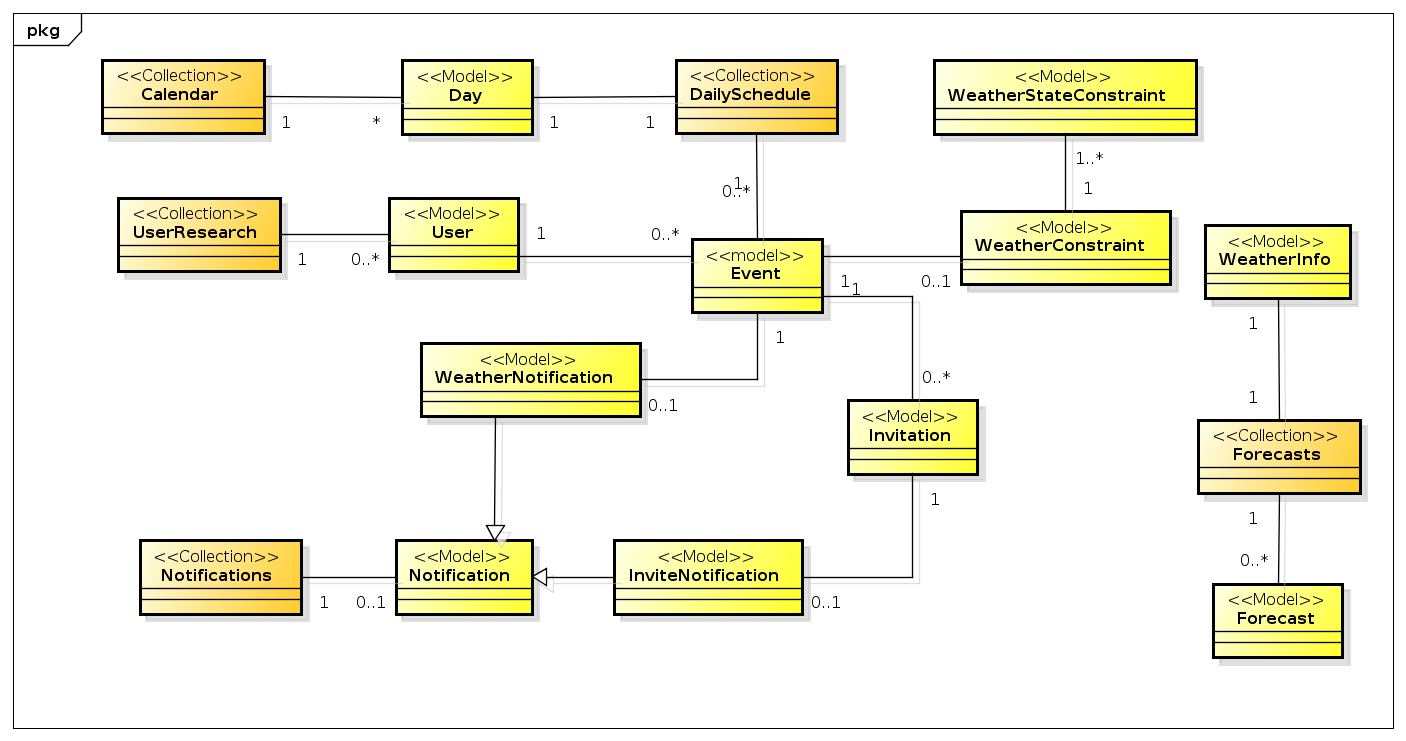
\includegraphics[width=1\textwidth]{../MVCDiagram/MVCBackbone/AllModelsAndCollections.png}
    \caption{Models and Collections}
     \label{fig:modelovervie}
     \end{figure}
   \end{center}  

\myparagraph{Show notifications}
In this diagram, as shown in figure~\ref{fig:notifMVC} there can be two types of notification\\
\begin{enumerate}
\item {\bf Invite notification}: it is the model representing a single notification of invite, giving the user the possibility to express his participation.
\item {\bf Weather notification}: it is used to tell the user whether there is an adverse condition for a future event and, if owner, ask for a date modification.
\end{enumerate}
Both these notification are extension of the generic \textbf{Notification}, which consists of a single element on the list of all the notifications. This model will be fetched from the server after performing some business intelligence operations over the \textit{"Participation"} entity for retrieving both the not answered invitations and the shortcoming events having possible weather issues.\\
The \textbf{Notifications} will be collected inside the omonimous collection.\\
The collection will be displayed using an \textit{ItemView} called \textit{NotificationView}, which will show the list of all the notifications in the user's webpage.
\begin{center}
 \begin{figure}[H]
    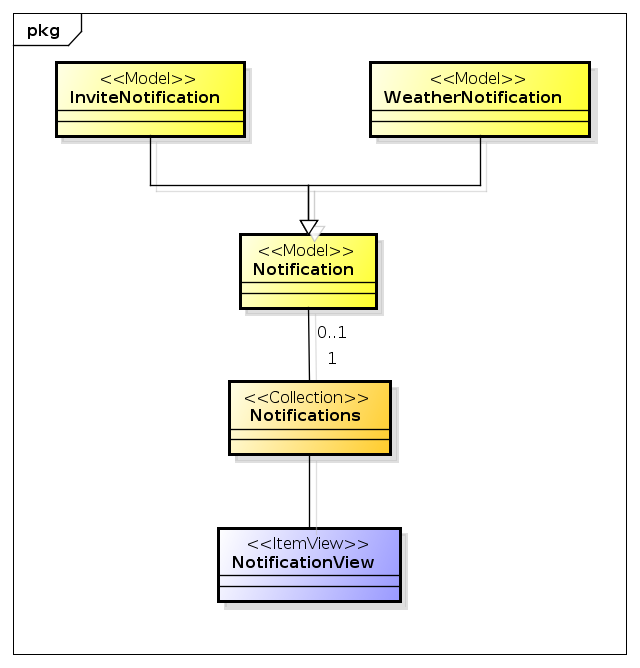
\includegraphics[width=1\textwidth]{../MVCDiagram/MVCBackbone/Notifications.png}
    \caption{Notifications}
     \label{fig:notifMVC}
     \end{figure}
   \end{center}
   
\myparagraph{Local forecast}
The user will be able to see the local forecast for the next days in a dedicated area of the website. This will be accomplished using the OpenWeatherMAP RESTful API from the client. The retrived data will be modeled in figure~\ref{fig:forecastMVC}.
The first model, called \textbf{WeatherInfo} will contain the metadata of the response, including the locality details.\\
The \textbf{Forecasts} will be then stored inside the omonimous collection, and each one will be modeled by \textbf{Forecast}. This model will contain the forecast information about a single interval. This collection will be rendered inside the \textbf{ForecastView} \textit{ItemView} which will be nested inside a box containing some of the data stored in the \textbf{WeatherInfo} model, managed by the \textbf{WeatherDataView} \textit{ItemView}.
\begin{center}
 \begin{figure}[H]
    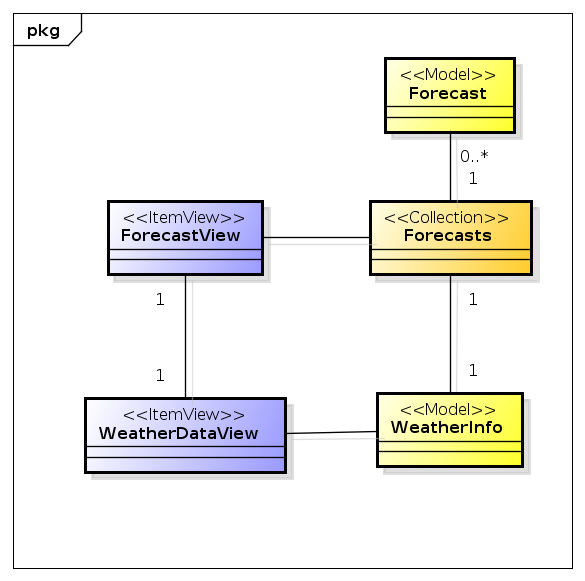
\includegraphics[width=1\textwidth]{../MVCDiagram/MVCBackbone/Forecast.png}
    \caption{Local forecast}
     \label{fig:forecastMVC}
     \end{figure}
   \end{center}
   
\myparagraph{Search Users}
The user will also be able to search other users, in order to find their profiles or invite them to an event. This will be realized, as illustrated in figure~\ref{fig:userSearchMVC}, from a \textbf{UserResearchView} which will list the users for a certain lookup keyword inputed by the user. As the user types the keyword, the \textbf{UserResearch} collection will be populated by \textbf{User} models, fetching them by the server.
\begin{center}
 \begin{figure}[H]
    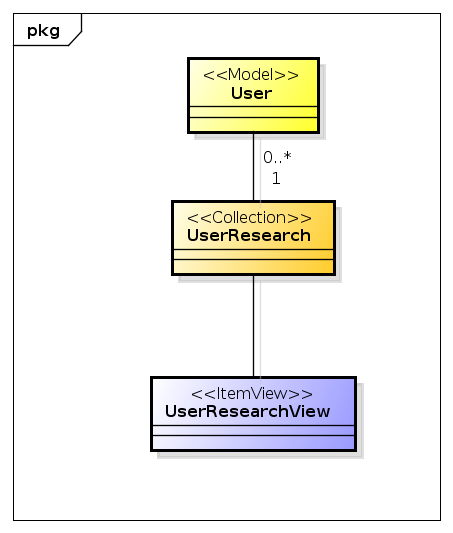
\includegraphics[width=1\textwidth]{../MVCDiagram/MVCBackbone/UserSearch.png}
    \caption{Search users}
     \label{fig:userSearchMVC}
     \end{figure}
   \end{center}
   
\myparagraph{User's calendar}
As the user will have a calendar to browse, data will be fetched asynchronously by intercepting the selection of a new period and rendering the related calendar and the events for that period. This task will be assigned to the model displayed in figure~
\ref{fig:calendarBCE}.
The \textbf{Calendar} collection will contain the list of \textbf{Day} models. The former will be displayed using a \textit{CollectionView} called \textbf{CalendarView}, which will be used for rendering every day. The rendering of the \textbf{Event} models, collected inside a \textbf{DailySchedule} collection will be accomplished by the \textbf{DayView}, which is an \textit{ItemView} nested inside the \textbf{CalendarView}. It will display the day and iterate over the events and display them inside in an apposite area related to that day.
\begin{center}
 \begin{figure}[H]
    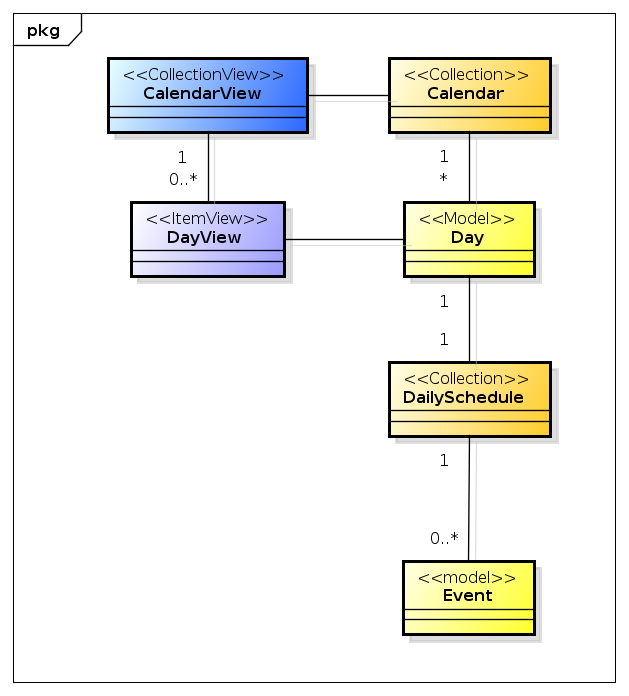
\includegraphics[width=1\textwidth]{../MVCDiagram/MVCBackbone/UserCalendar.png}
    \caption{Calendar period change}
     \label{fig:calendarBCE}
     \end{figure}
   \end{center}  

\subsection{Sequence Diagram}
\subsubsection{Server-side BCE}
In this section we'll show some sequence diagram associated with the BCE Diagram explained in ~\ref{sec:BCE} section in order to give  a more comprehensive overview either of the BCE patterns and of course of our system behavior.
\myparagraph{Sign Up}
Figure ~\ref{fig:signupSeq} shows the process for the registration of a new user into the system. As a user accesses the system through the MainPage, he will reach either the login or the register form to the system. If the user wants to register this is what happens.
The user will submit his information through the form and the SignUpController will check that the correctness of the value. If these information are valid then a new user will be created by the SignUpController and inserted in to the system else if the information are not correct a excepetion is thrown and the registration fails. 
\begin{center}
 \begin{figure}[H]
    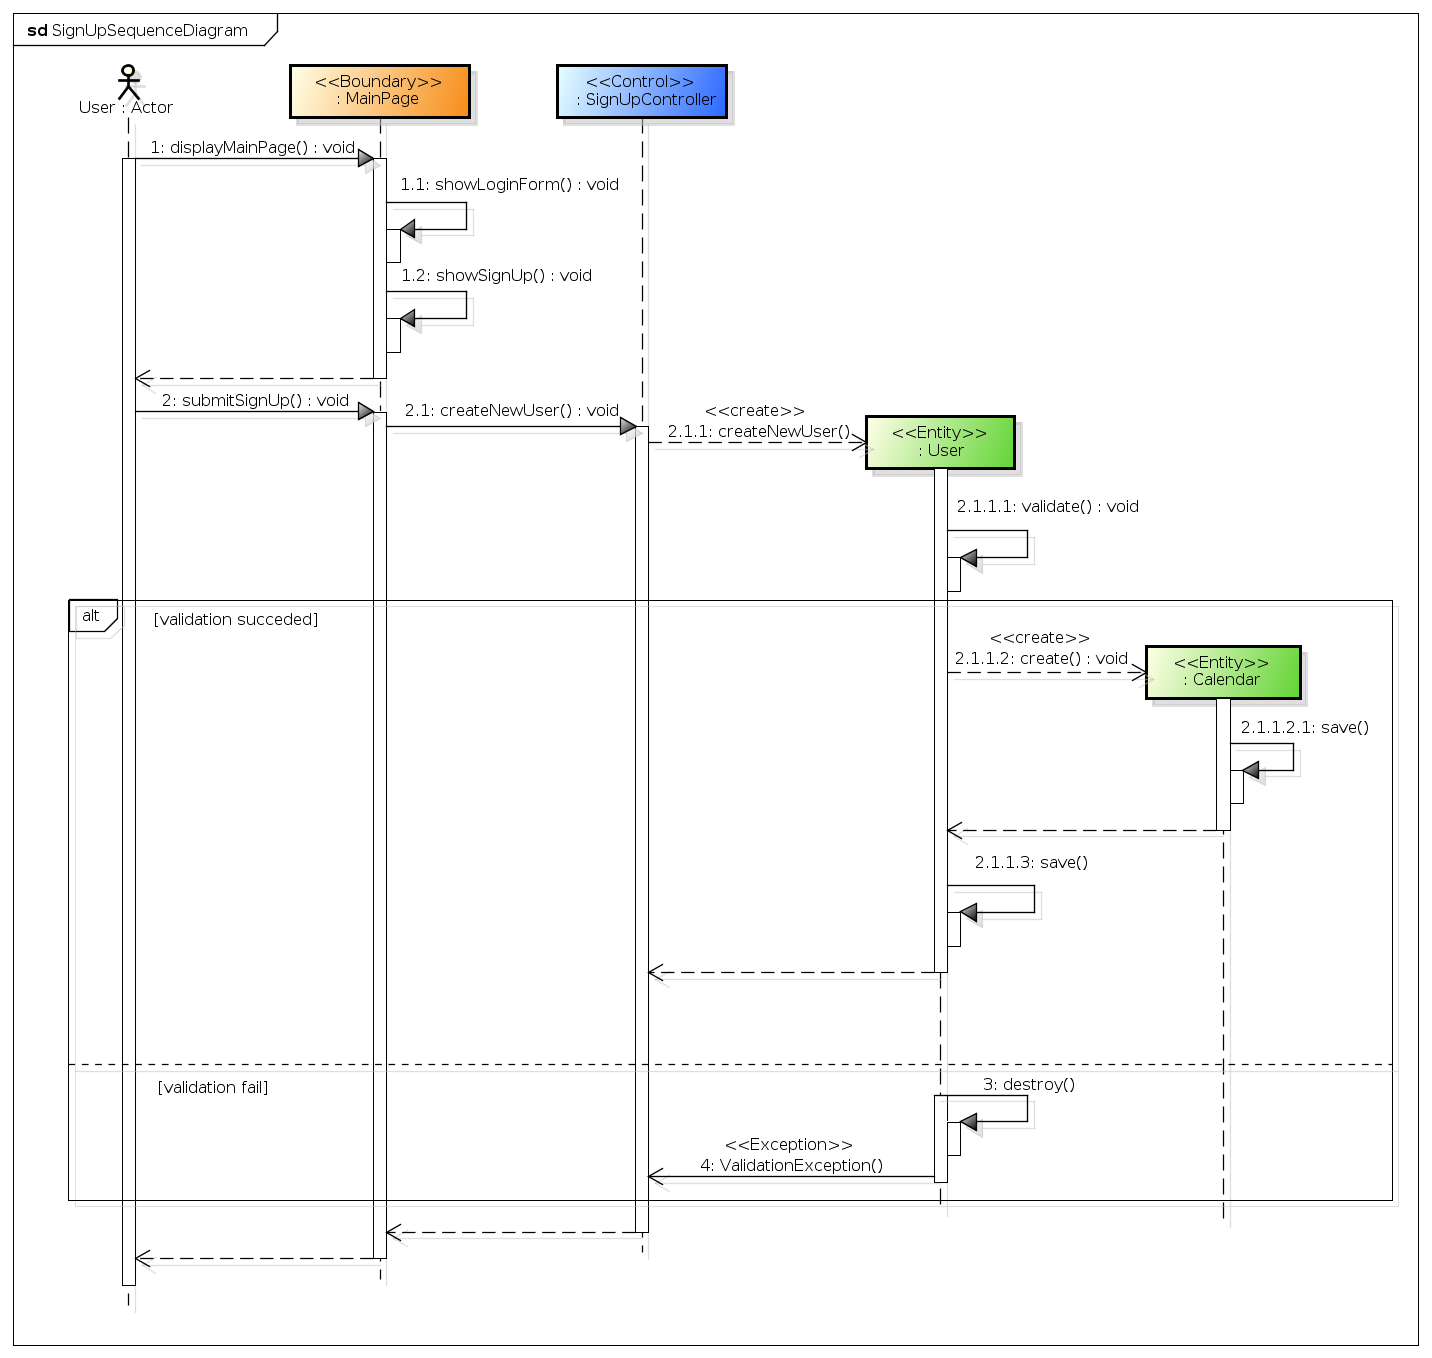
\includegraphics[width=0.9\textwidth]{../BCEDiagram/BCE/EntityOverview/SignUpSequenceDiagram.png}
    \caption{Sign up sequence diagram}
     \label{fig:signupSeq}
     \end{figure}
   \end{center}  
  
  \myparagraph{Log In}
  The diagrams represented in figure ~\ref{fig:Login1Seq}  and ~\ref{fig:Login2Seq} describe the login phase for a registered user in the system. As the user enters the platform the login form is shown to him and the validation process begins. The whole sequence diagram is divided in two part in order to  give a better understanding of it.\\
  The first diagram fig.~\ref{fig:Login1Seq} refers to the validation of an user. After he submitted his login value, from the log in form in the MainPage, the LoginController verify the validity of these information, in case of an affermative response then the user is authenticated in to the system and he is redirect to the UserPage where thanks to CalendarController his calendar is loaded and shown.
  \begin{center}
 \begin{figure}[H]
    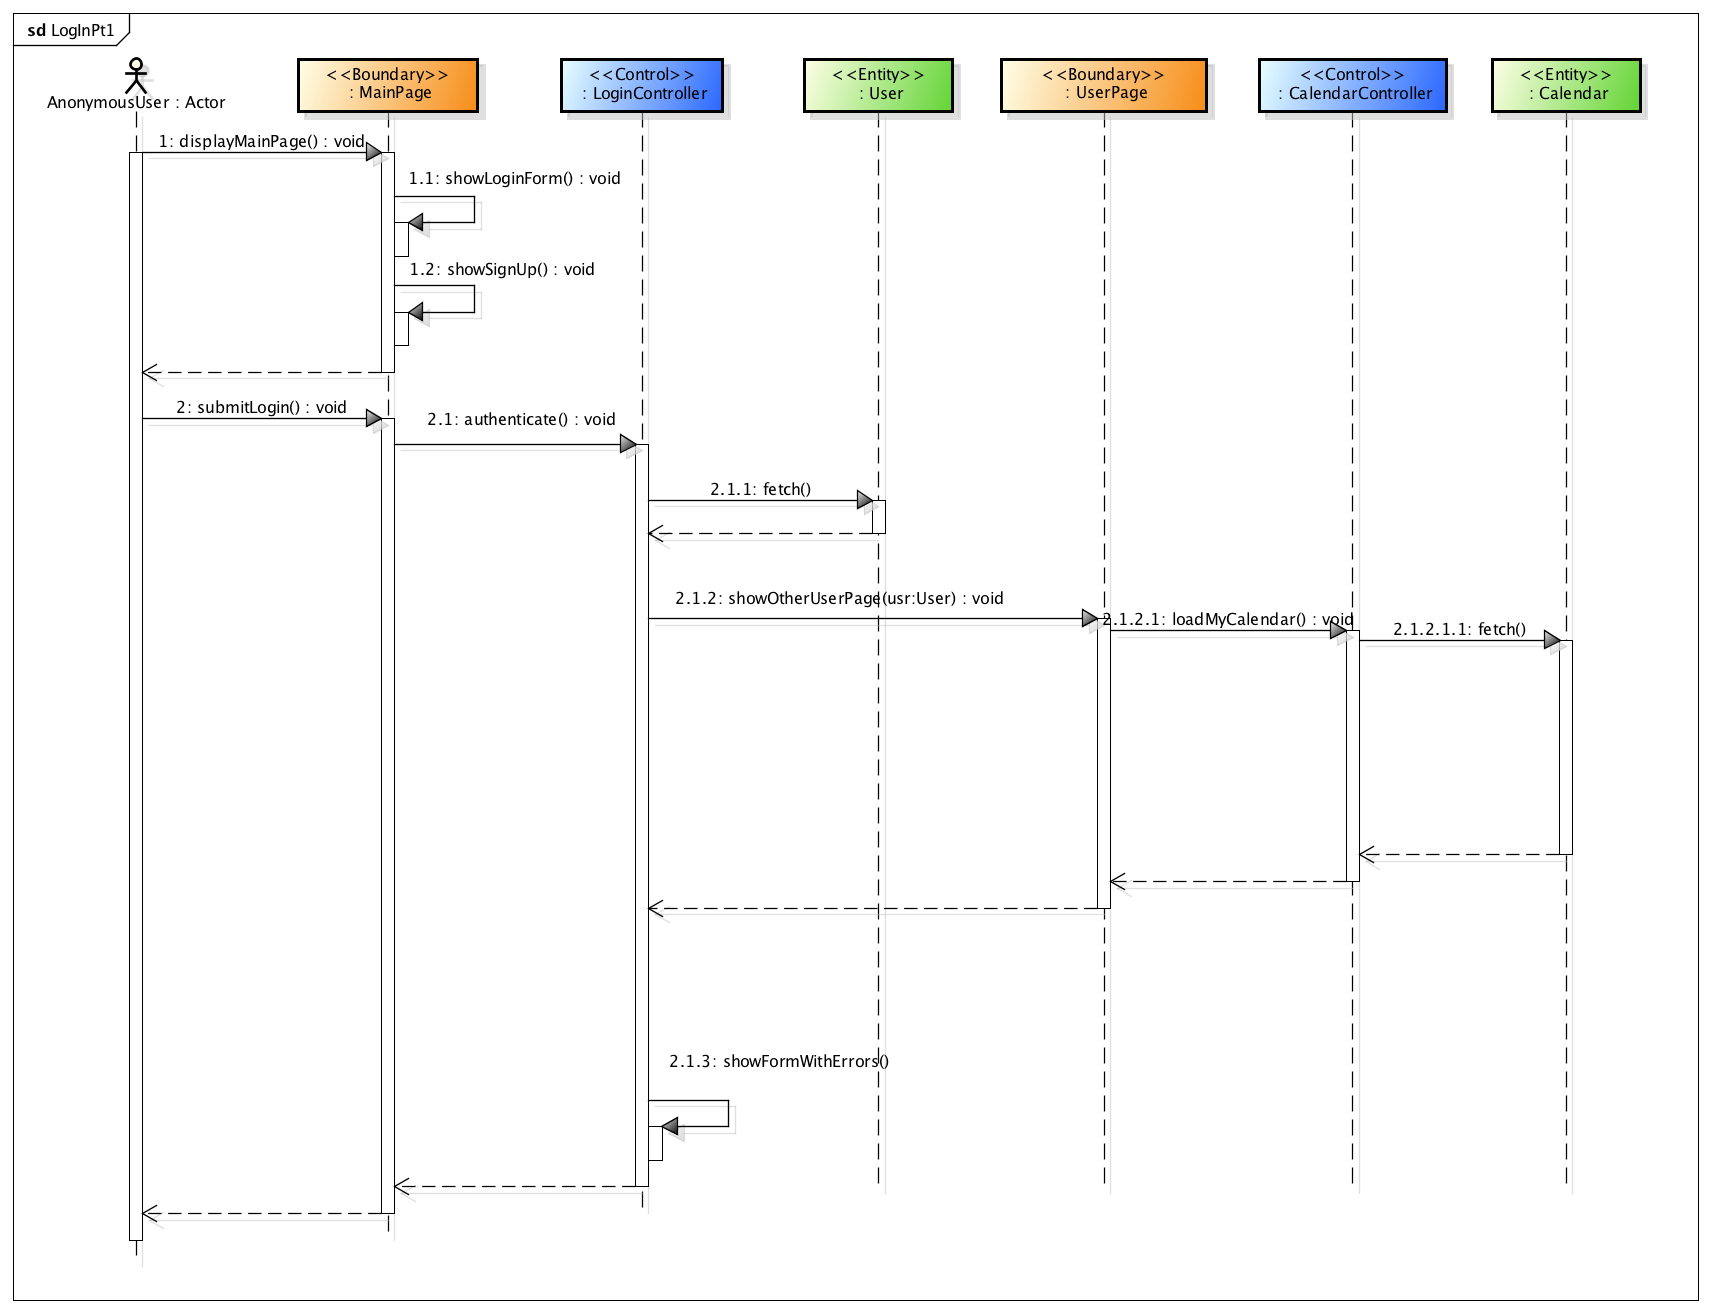
\includegraphics[width=0.9\textwidth]{../BCEDiagram/BCE/EntityOverview/LogInPt1.png}
    \caption{Login part 1}
     \label{fig:Login1Seq}
     \end{figure}
   \end{center}  
     \begin{center}
So if the diagram~\ref{fig:Login1Seq} represents the authentication process of an user then the diagram~\ref{fig:Login2Seq} represents the process used by the system to load the event related to the user's calendar. Once the user is logged in, he can see all the events which owns, all the events in which was invited or all the events that is going to attend. 
 \begin{figure}[H]
    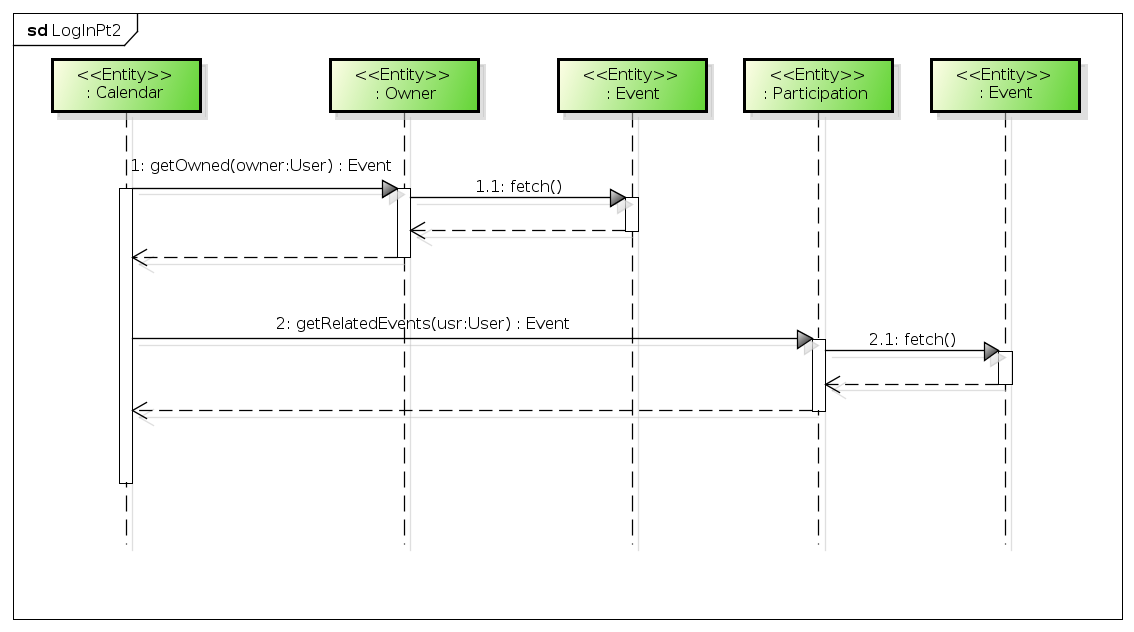
\includegraphics[width=1\textwidth]{../BCEDiagram/BCE/EntityOverview/LogInPt2.png}
    \caption{Login part 2}
     \label{fig:Login2Seq}
     \end{figure}
   \end{center} 
 \myparagraph{New Event}
 The diagram represented in figure ~\ref{fig:newEveSeq} shows how an user will create a new event and customize it as he wants. The NewModifyEventPage will show to him an empty form to fill with the desired value for the event such as the date, the place, the invited user or the weather constraint. The same form is shown to an user that wants to see the event's details and eventually ,if he's also its owner, to modify the current value.
Therefore after an user creates or modifies an event, the EventController check that all the values are correct and then either creates a new event or modify an existing one or, if the submitted preferences are not valid, it throws an exception and the creation process fails.  
  \begin{center}
 \begin{figure}[H]
    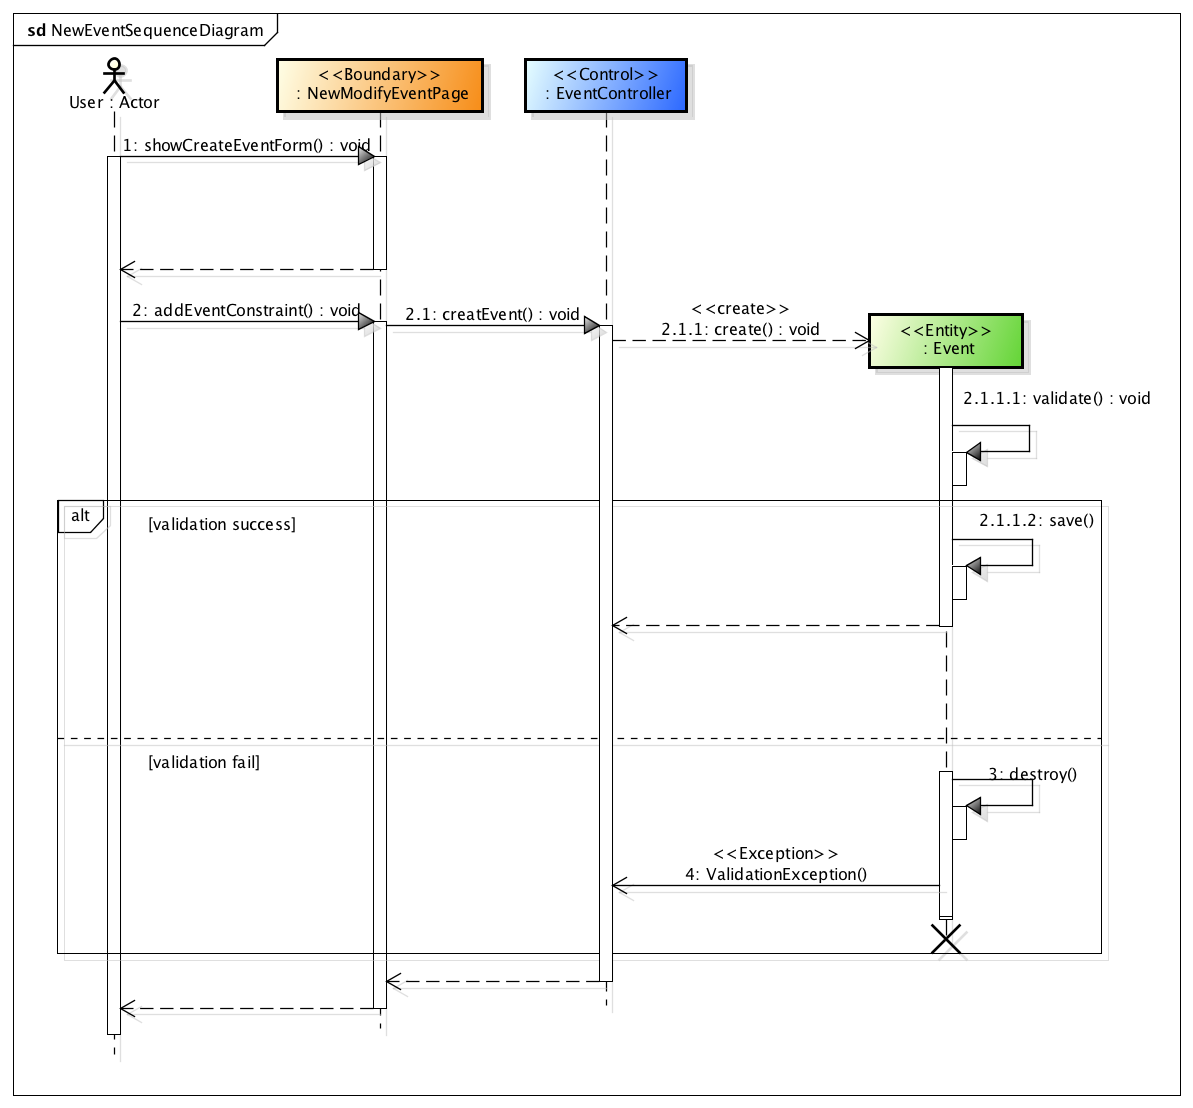
\includegraphics[width=1\textwidth]{../BCEDiagram/BCE/EntityOverview/NewEventSequenceDiagram.png}
    \caption{New event sequence Diagram}
     \label{fig:newEveSeq}
     \end{figure}
   \end{center} 
\myparagraph{Search Users}
The diagram in figure ~\ref{fig:searchusSeq} shows the behavior of the system when an user searches for an other user's agenda. The searching and the loading process of the target calendar is accomplished by the CalendarController which once it finds the calendar and makes sure that it was marked visible to everyone by its owner, it fetches all the event related to it, taking care to filter the public event and the private one and finally shows to the user only the public event of the desired user.
 \begin{center}
 \begin{figure}[H]
    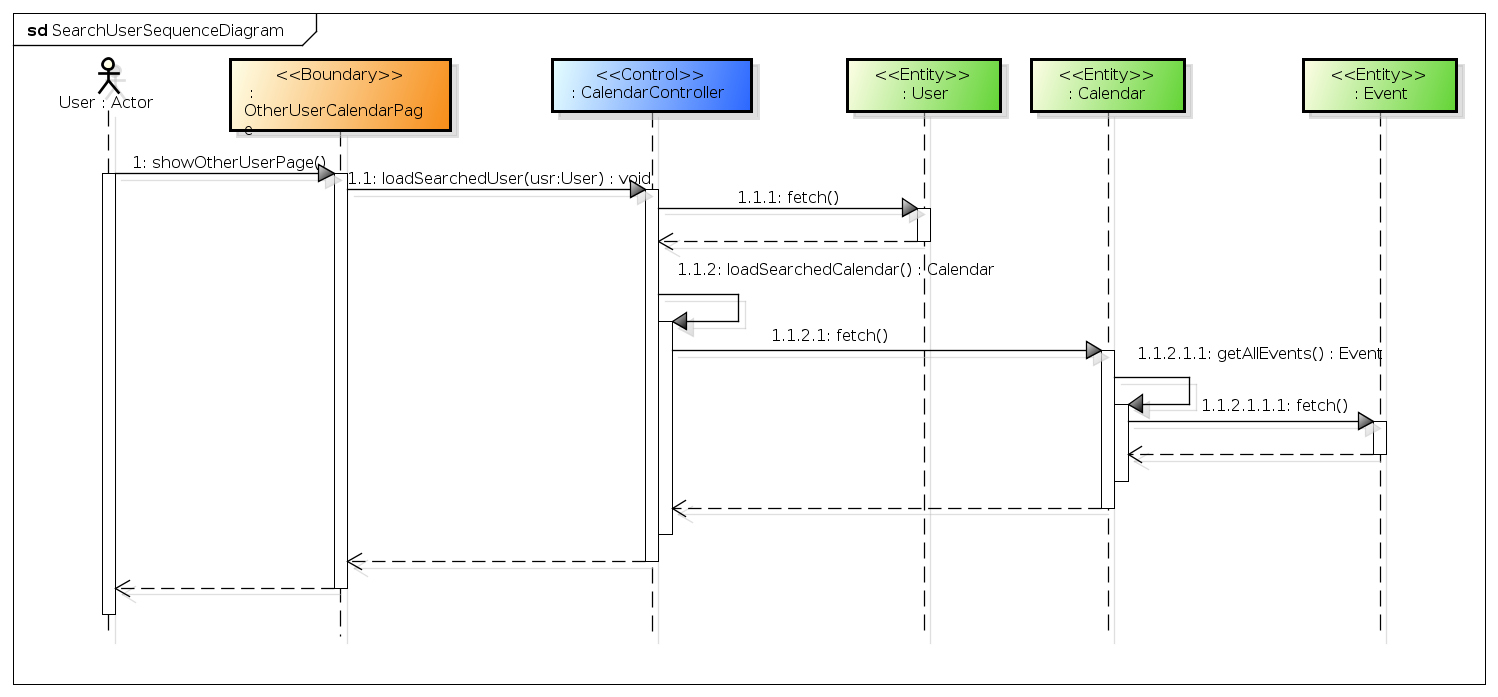
\includegraphics[width=1\textwidth]{../BCEDiagram/BCE/EntityOverview/SearchUserSequenceDiagram.png}
    \caption{Search users sequence diagram}
     \label{fig:searchusSeq}
     \end{figure}
   \end{center} 
\subsubsection{Client-side MVC}
\myparagraph{Load notifications}
The diagram in figure ~\ref{fig:loadnotifSeq} shows the behavior of the client application when a user logs onto the platform. As the web page loads, the application will fetch from the server the list of the notifications for that user. After that, each notification is displayed to the user.
 \begin{center}
 \begin{figure}[H]
    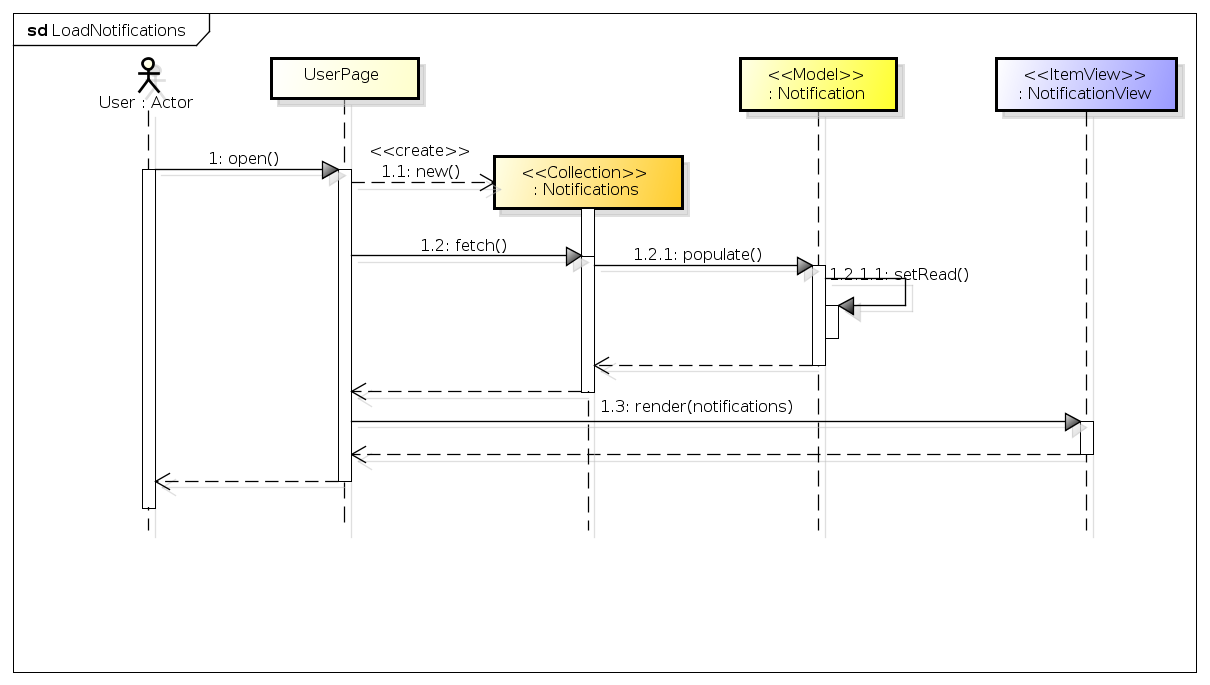
\includegraphics[width=1\textwidth]{../MVCDiagram/MVCBackbone/LoadNotifications.png}
    \caption{Load notifications sequence diagram}
     \label{fig:loadnotifSeq}
     \end{figure}
   \end{center} 
   
\myparagraph{Local forecast}
Figure ~\ref{fig:forecasteq} illustrates how the local forecast is loaded as the user opens his calendar. The user fetches the forecast for the current locality storing it inside a nested model and collection structure. After this process, this structure is rendered in a dedicated area. The \textbf{WeatherDataView} will be involved in displaying the metadata of the forecast, like the locality for which the forecast is shown. This view will also contain the \textbf{ForecastView}, a view for displaying the list of all the forecast periods.
 \begin{center}
 \begin{figure}[H]
    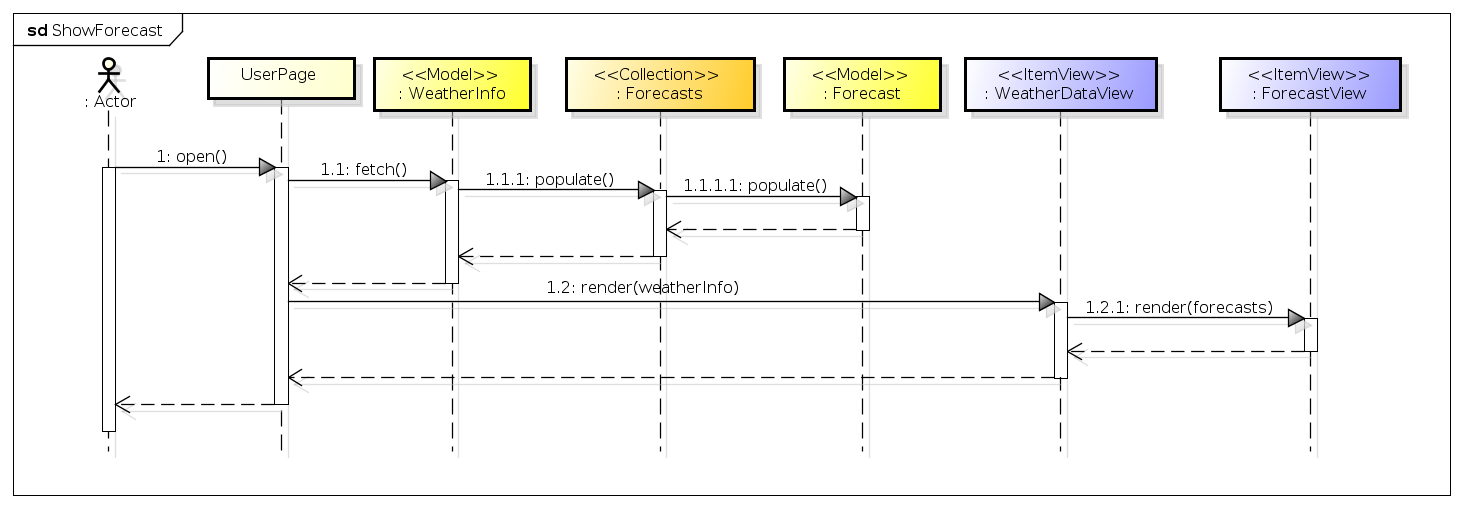
\includegraphics[width=1\textwidth]{../MVCDiagram/MVCBackbone/ShowForecast.png}
    \caption{Show Forecast sequence diagram}
     \label{fig:forecasteq}
     \end{figure}
   \end{center} 
   
\myparagraph{Search user}
The diagram in figure~\ref{fig:searchuseq} shows how an user can reach and view other user agenda. The system will fetch the searched user data corresponding with the string submitted by the user and then will store that data into a nested model. The {\bf UserResearchView} will display all the user that match with the searched string. 
    \begin{center}
 \begin{figure}[H]
    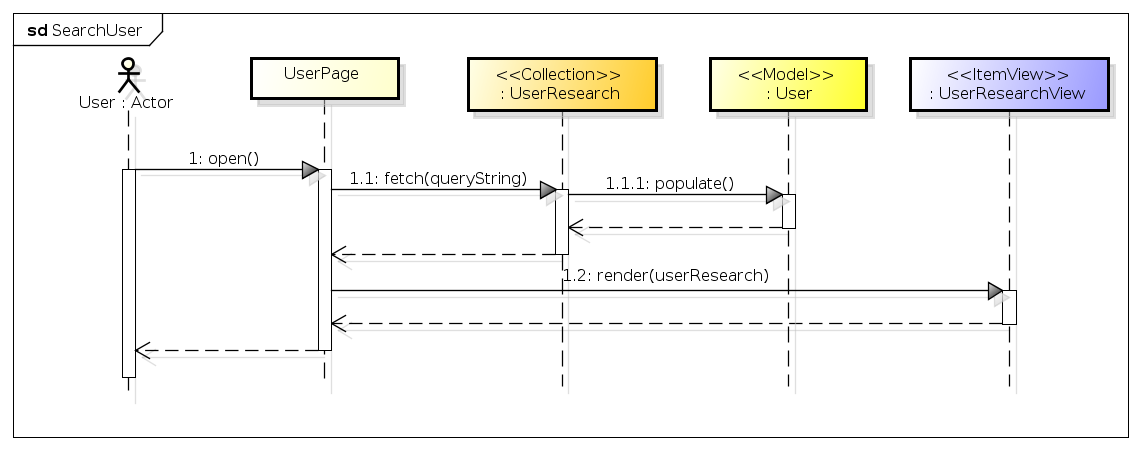
\includegraphics[width=1\textwidth]{../MVCDiagram/MVCBackbone/SearchUser.png}
    \caption{Search user sequence diagram}
     \label{fig:searchuseq}
     \end{figure}
   \end{center} 
\myparagraph{User's calendar}
The figure~\ref{fig:usercalese} illustrates how an user can change the date range shown by the calendar. After an user select a different date's period to be displayed, the system takes care of fetching this selected period and then it will populate a model and a collection  structure, whereupon the {\bf CalendarView} render the new calendar with the metadata of the selected date range while the {\bf DayView} will display the daily schedule.
 \begin{center}
 \begin{figure}[H]
    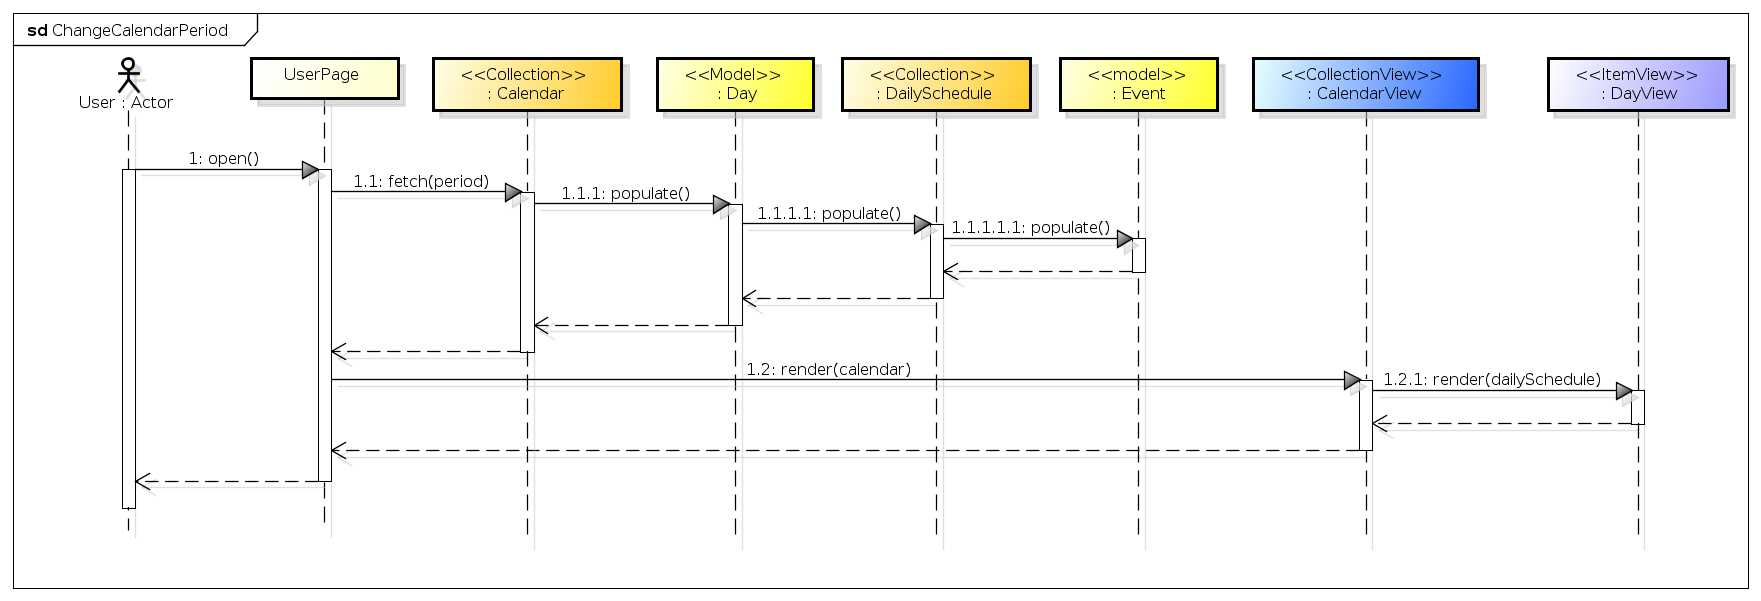
\includegraphics[width=1\textwidth]{../MVCDiagram/MVCBackbone/ChangeCalendarPeriod.png}
    \caption{Change calendar period sequence diagram}
     \label{fig:usercalese}
     \end{figure}
   \end{center} 
